\section{The TensorFlow Programming Model}\label{sec:model}

In this section we provide an in-depth discussion of the abstract computational
principles underlying the TensorFlow software library. We begin with a thorough
examination of the basic structural and architectural decisions made by the
TensorFlow development team and explain how machine learning algorithms may be
expressed in its dataflow graph language. Subsequently, we study TensorFlow's
execution model and provide insight into the way TensorFlow graphs are assigned
to available hardware units in a local as well as distributed environment. Then,
we investigate the various optimizations incorporated into TensorFlow, targeted
at improving both software and hardware efficiency. Lastly, we list extensions
to the basic programming model that aid the user in both computational as well
as logistical aspects of training a machine learning model with TensorFlow.

\subsection{Computational Graph Architecture}\label{sec:model-graphs}

In TensorFlow, machine learning algorithms are represented as
\emph{computational graphs}. A computational or \emph{dataflow} graph is a form
of directed graph where \emph{vertices} or \emph{nodes} describe operations,
while \emph{edges} represent data flowing between these operations. If an output
variable $z$ is the result of applying a binary operation to two inputs $x$ and
$y$, then we draw directed edges from $x$ and $y$ to an output node representing
$z$ and annotate the vertex with a label describing the performed
computation. Examples for computational graphs are given in Figure
\ref{fig:graphs}. The following paragraphs discuss the principle elements of
such a dataflow graph, namely \emph{operations}, \emph{tensors},
\emph{variables} and \emph{sessions}.

\begin{figure}
  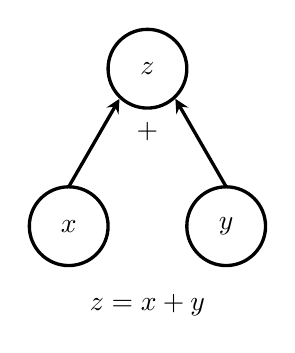
\begin{tikzpicture}
    % Result
    \draw [very thick] (1, 2) circle [radius=0.5cm] node {$z$};

    % Input Nodes
    \draw [very thick] (0, 0) circle [radius=0.5cm] node {$x$};
    \draw [very thick] (2, 0) circle [radius=0.5cm] node {$y$};

    % Edges
    \draw [very thick, -stealth] (0, 0.5) -- ++(60:1.29);
    \draw [very thick, -stealth] (2, 0.5) -- ++(120:1.29);

    % Operation Label
    \draw (1, 1.2) node {$+$};

    % Figure Label
    \draw (1, -1) node {$z = x + y$};
  \end{tikzpicture}
  %
  \hspace{0.2cm}
  %
  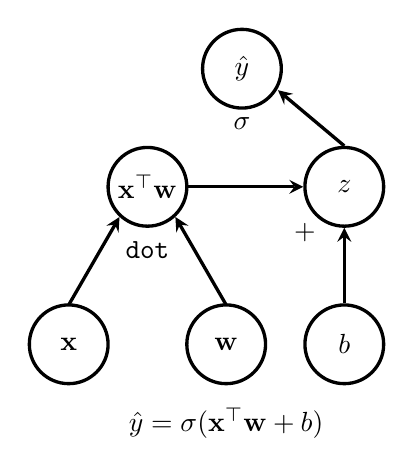
\begin{tikzpicture}
    % x^T w
    \draw [very thick] (1, 2) circle [radius=0.5cm] node {$\mathbf{x^\top w}$};

    % x and weights
    \draw [very thick] (0, 0) circle [radius=0.5cm] node {$\mathbf{x}$};
    \draw [very thick] (2, 0) circle [radius=0.5cm] node {$\mathbf{w}$};

    % Edges
    \draw [very thick, -stealth] (0, 0.5) -- ++(60:1.29);
    \draw [very thick, -stealth] (2, 0.5) -- ++(120:1.29);

    % Operation Label
    \draw (1, 1.2) node {\texttt{dot}};

    % Bias
    \draw [very thick] (3.5, 0) circle [radius=0.5cm] node {$b$};

    % z = (x^T w) + b
    \draw [very thick] (3.5, 2) circle [radius=0.5cm] node {$z$};

    % Operation label
    \draw (3, 1.42) node {$+$};

    % Edges
    \draw [very thick, -stealth] (3.5, 0.52) -- (3.5, 1.48);
    \draw [very thick, -stealth] (1.52, 2) -- (2.98, 2);

    % Sigmoid
    \draw [very thick] (2.2, 3.5) circle [radius=0.5] node {$\hat{y}$};

    % Operation label
    \draw (2.2, 2.8) node {$\sigma$};

    % Edge
    \draw [very thick, -stealth] (3.5, 2.52) -- ++(140:1.1cm);


    % Figure Label
    \draw (2, -1) node {$\hat{y} = \sigma(\mathbf{x}^\top \mathbf{w} + b)$};
  \end{tikzpicture}
  \caption{Examples of computational graphs. The left graph displays a very
    simple computation, consisting of just an addition of the two input
    variables $x$ and $y$. In this case, $z$ is the result of the operation $+$,
    as the annotation suggests. The right graph gives a more complex example of
    computing a logistic regression variable $\hat{y}$ in for some example
    vector $\mathbf{x}$, weight vector $\mathbf{w}$ as well as a scalar bias
    $b$. As shown in the graph, $\hat{y}$ is the result of the \emph{sigmoid} or
    \emph{logistic} function $\sigma$.}
  \label{fig:graphs}
\end{figure}

\subsubsection{Operations}\label{sec:model-graphs-ops}

The major benefit of representing an algorithm in form of a graph is not only
the intuitive (visual) expression of dependencies between units of a
computational model, but also the fact that the definition of a \emph{node}
within the graph can be kept very general. In TensorFlow, nodes represent
\emph{operations}, which in turn express the combination or transformation of
data flowing through the graph \cite{tensorflow}. An operation can have
\emph{zero or more} inputs and produce \emph{zero or more} outputs. As such, an
operation may represent a mathematical equation, a variable or constant, a
control flow directive, a file I/O operation or even a network communication
port. It may seem unintuitive that an operation, which the reader may associate
with a \emph{function} in the mathematical sense, can represent a constant or
variable. However, a constant may be thought of as an operation that takes no
inputs and always produces the same output corresponding to the constant it
represents. Analogously, a variable is really just an operation taking no input
and producing the current state or value of that variable. Table \ref{tab:ops}
gives an overview of different kinds of operations that may be declared in a
TensorFlow graph.

\begin{table}[b!]
  \begin{tabular}{ll}
    \textbf{Category} & \textbf{Examples}
    \\ \toprule
    Element-wise operations & \texttt{Add}, \texttt{Mul}, \texttt{Exp}
    \\
    Matrix operations & \texttt{MatMul}, \texttt{MatrixInverse}
    \\
    Value-producing operations & \texttt{Constant}, \texttt{Variable}
    \\
    Neural network units & \texttt{SoftMax}, \texttt{ReLU}, \texttt{Conv2D}
    \\
    Checkpoint operations & \texttt{Save}, \texttt{Restore}
    \\ \bottomrule
    \end{tabular}
    \label{tab:ops}
    \caption{Examples for TensorFlow operations \cite{tensorflow}.}
\end{table}

Any operation must be backed by an associated implementation. In
\cite{tensorflow} such an implementation is referred to as the operation's
\emph{kernel}. A particular kernel is always specifically built for execution on
a certain kind of device, such as a CPU, GPU or other hardware unit.

\subsubsection{Tensors}\label{sec:model-graphs-tensors}

In TensorFlow, edges represent data flowing from one operation to another and
are referred to as \emph{tensors}. A tensor is a multi-dimensional collection of
homogeneous values with a fixed, static type. The number of dimensions of a
tensor is termed its \emph{rank}. A tensor's \emph{shape} is the tuple
describing its size, i.e. the number of components, in each dimension. In the
mathematical sense, a tensor is the generalization of two-dimensional matrices,
one-dimensional vectors and also scalars, which are simply tensors of rank zero.

In terms of the computational graph, a tensor can be seen as a \emph{symbolic
  handle} to one of the outputs of an operation. A tensor itself does not hold
or store values in memory, but provides only an interface for retrieving the
value referenced by the tensor. When creating an operation in the TensorFlow
programming environment, such as for the expression $x + y$, a tensor object is
returned. This tensor may then be supplied as input to other computations,
thereby connecting the source and destination operations with an edge. By these
means, data flows through a TensorFlow graph.

Next to regular tensors, TensorFlow also provides a \texttt{SparseTensor}
data structure, allowing for a more space-efficient dictionary-like
representation of \emph{sparse tensors} with only few non-zeros entries.

\subsubsection{Variables}\label{sec:model-graphs-vars}

In a typical situation, such as when performing stochastic gradient descent
(SGD), the graph of a machine learning model is executed from start to end
multiple times for a single experiment. Between two such invocations, the
majority of tensors in the graph are destroyed and do not persist. However, it
is often necessary to maintain state across evaluations of the graph, such as
for the weights and parameters of a neural network. For this purpose, there
exist \emph{variables} in TensorFlow, which are simply special operations that
can be added to the computational graph.

In detail, variables can be described as persistent, mutable handles to
in-memory buffers storing tensors. As such, variables are characterized by a
certain shape and a fixed type. To manipulate and update variables, TensorFlow
provides the \texttt{assign} family of graph operations.

When creating a variable node for a TensorFlow graph, it is necessary to supply
a tensor with which the variable is initialized upon graph execution. The shape
and data type of the variable is then deduced from this
initializer. Interestingly, the variable itself does not store this initial
tensor. Rather, constructing a variable results in the addition of \emph{three}
distinct nodes to the graph:

\begin{enumerate}
  \item The actual variable node, holding the mutable state.
  \item An operation producing the initial value, often a constant.
  \item An \emph{initializer} operation, that \texttt{assign}s the initial value
    to the variable tensor upon evaluation of the graph.
\end{enumerate}

An example for this is given in Figure \ref{fig:variable}.

\begin{figure}
  \centering
    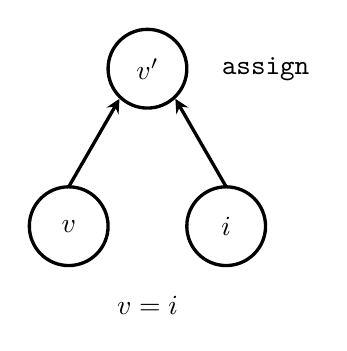
\begin{tikzpicture}
    % Result
    \draw [very thick] (1, 2) circle [radius=0.5cm] node {$v'$};

    % Input Nodes
    \draw [very thick] (0, 0) circle [radius=0.5cm] node {$v$};
    \draw [very thick] (2, 0) circle [radius=0.5cm] node {$i$};

    % Edges
    \draw [very thick, -stealth] (0, 0.5) -- ++(60:1.29);
    \draw [very thick, -stealth] (2, 0.5) -- ++(120:1.29);

    % Operation Label
    \draw (2.5, 2) node {\texttt{assign}};

    % Figure Label
    \draw (1, -1) node {$v = i$};
  \end{tikzpicture}
  \caption{The three nodes that are added to the computational graph for every
    variable definition. The first, $v$, is the variable operation that holds a
    mutable in-memory buffer containing the value tensor of the variable. The
    second, $i$, is the node producing the initial value for the variable, which
    can be any tensor. Lastly, the \texttt{assign} node will set the variable to
    the initializer's value when executed. The \texttt{assign} node also
    produces a tensor referencing the initialized value $v'$ of the variable,
    such that it may be connected to other nodes as necessary (e.g. when using a
    variable as the initializer for another variable).}
  \label{fig:variable}
\end{figure}

\subsubsection{Sessions}\label{sec:model-graphs-sessions}

In TensorFlow, the execution of operations and evaluation of tensors may only be
performed in a special environment referred to as \emph{session}. One of the
responsibilities of a session is to encapsulate the allocation and management of
resources such as variable buffers. Moreover, the \texttt{Session} interface of
the TensorFlow library provides a \texttt{run} routine, which is the primary
entry point for executing parts or the entirety of a computational graph. This
method takes as input the nodes in the graph whose tensors should be computed
and returned. Moreover, an optional mapping from arbitrary nodes in the graph to
respective replacement values --- referred to as \emph{feed nodes} --- may be
supplied to \texttt{run} as well \cite{tensorflow}.

Upon invocation of \texttt{run}, TensorFlow will start at the requested output
nodes and work backwards, examining the graph dependencies and computing the
full transitive closure of all nodes that must be executed. These nodes may then
be assigned to one or many physical execution units (CPUs, GPUs etc.) on one or
many machines. The rules by which this assignment takes place are determined by
TensorFlow's \emph{placement algorithm}, discussed in detail in Subsection
\ref{subsec:model-exec}. Furthermore, as there exists the possibility to specify
explicit orderings of node evaluations, called \emph{control dependencies}, the
execution algorithm will ensure that these dependencies are maintained.

\subsection{Execution Model}\label{sec:model-exec}

To execute computational graphs composed of the various elements just discussed,
TensorFlow divides the tasks for its implementation among four distinct groups:
the \emph{client}, the \emph{master}, a set of \emph{workers} and lastly a
number of \emph{devices}. When the client requests evaluation of a TensorFlow
graph via a \texttt{Session}'s \texttt{run} routine, this query is sent to the
master process, which in turn delegates the task to one or more worker processes
and coordinates their execution. Each worker is subsequently responsible for
overseeing one or more devices, which are the physical processing units for
which the kernels of an operation are implemented.

Within this model, there are two degrees of scalability. The first degree
pertains to scaling the number of machines on which a graph is executed. The
second degree refers to the fact that on each machine, there may then be more
than one device, such as, for example, five independent GPUs and/or three
CPUs. For this reason, there exist two ``versions'' of TensorFlow, one for local
execution on a single machine (but possibly many devices), and one supporting a
\emph{distributed} implementation across many machines and many devices. Figure
\ref{fig:exec} visualizes a possible distributed setup. While the initial
release of TensorFlow supported only single-machine execution, the distributed
version was open-sourced on April 13, 2016 \cite{tensorflowdist}.

\begin{figure}
  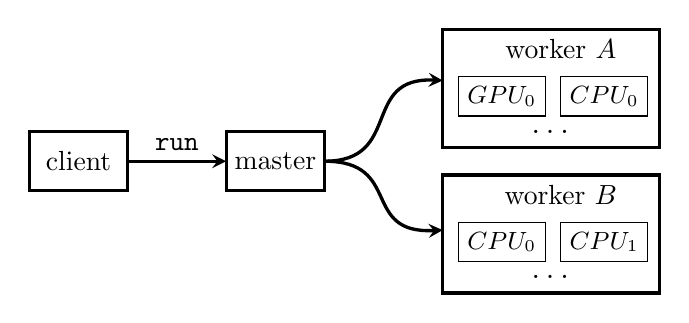
\begin{tikzpicture}
    % Client
    \draw [very thick] (0, 0) rectangle ++(1.25, 0.75) node [midway] {client};

    % Master
    \draw [very thick] (2.5, 0) rectangle ++(1.25, 0.75) node [midway] {master};
    \draw [very thick, -stealth] (1.25, 0.375) -- (2.5, 0.375) node [midway,
    above] {\texttt{run}};

    % Worker 1
    \draw [very thick] (5.25, 0.55) rectangle ++(2.75, 1.5);
    \draw (6.75, 1.8) node {worker $A$};
    \draw (5.45, 0.95) rectangle ++(1.1, 0.5) node [midway] {\small$GPU_0$};
    \draw (6.75, 0.95) rectangle ++(1.1, 0.5) node [midway] {\small$CPU_0$};
    \draw (6.65, 0.75) node {\large\dots};


    % Worker 2
    \draw [very thick] (5.25, -1.3) rectangle ++(2.75, 1.5);
    \draw (6.75, -0.05) node {worker $B$};
    \draw (5.45, -0.9) rectangle ++(1.1, 0.5) node [midway] {\small$CPU_0$};
    \draw (6.75, -0.9) rectangle ++(1.1, 0.5) node [midway] {\small$CPU_1$};
    \draw (6.65, -1.1) node {\large\dots};

    % Edges
    \draw [very thick, -stealth]
          (3.75, 0.375) .. controls +(1, 0) and (4.2, 1.45) .. (5.25, 1.4);
    \draw [very thick, -stealth]
          (3.75, 0.375) .. controls +(1, 0) and (4.2, -0.55) .. (5.25, -0.5);

  \end{tikzpicture}
  \caption{A visualization of the different execution agents in a multi-machine,
    multi-device hardware configuration.}
  \label{fig:exec}
\end{figure}

\subsubsection{Devices}\label{sec:model-exec-devices}

Devices are the smallest, most basic entities in the TensorFlow execution
model. All nodes in the graph, that is, the kernel of each operation, must
eventually be mapped to an available device to be executed. In practice, a
device will most often be either a CPU or a GPU. However, TensorFlow supports
registration of further kinds of physical execution units by the user. For
example, in May 2016, Google announced its \emph{Tensor Processing Unit} (TPU),
a custom built ASIC (application-specific-integrated-circuit) optimized
specifically for fast tensor computations \cite{tpu}. It is thus understandably
easy to integrate new device classes as novel hardware emerges.

To oversee the evaluation of nodes on a device, a worker process is spawned by
the master. As a worker process may manage one or many devices on a single
machine, a device is identified not only by a name, but also an index for its
worker group. For example, the first CPU in a particular group may be identified
by the string ``/cpu:0''.

\subsubsection{Placement Algorithm}\label{sec:model-exec-placement}

To determine what nodes to assign to which device, TensorFlow makes use of a
\emph{placement algorithm}. The placement algorithm simulates the execution of
the computational graph and traverses its nodes from input tensors to output
tensors. To decide on which of the available devices
$\mathbb{D} = \{d_1, \dots, d_n\}$ to place a given node $\nu$ encountered
during this traversal, the algorithm consults a \emph{cost model}
$C_\nu(d)$. This cost model takes into account four pieces of information to
determine the optimal device $\hat{d} = \argmin_{d \in \mathbb{D}} C_\nu(d)$ on
which to place the node during execution:

\begin{enumerate}
  \item Whether or not there exists an implementation (kernel) for a node on the
    given device at all. For example, if there is no GPU kernel for a particular
    operation, any GPU device would automatically incur an infinite cost.
  \item Estimates of the size (in bytes) for a node's input and output tensors.
  \item The expected execution time for the kernel on the device.
  \item A heuristic for the cost of cross-device (and possibly cross-machine)
    transmission of the input tensors to the operation, in the case that the
    input tensors have been placed on nodes different from the one currently
    under consideration.
\end{enumerate}

\subsubsection{Cross-Device Execution}\label{sec:model-exec-single}

If the hardware configuration of the user's system provides more than one
device, the placement algorithm will often distribute a graph's nodes among
these devices. This can be seen as partitioning the set of nodes into classes,
one per device. As a consequence, there may be cross-device dependencies between
nodes that must be handled via a number of additional steps. Let us consider for
this two devices $A$ and $B$ with particular focus on a node $\nu$ on device
$A$. If $\nu$'s output tensor forms the input to some other operations
$\alpha, \beta$ on device $B$, there initially exist cross-device edges
$\nu \rightarrow \alpha$ and $\nu \rightarrow \beta$ from device $A$ to device
$B$. This is visualized in Figure \ref{fig:cross-a}.

In practice, there must be some means of transmitting $\nu$'s output tensor from
$A$, say a GPU device, to $B$ --- maybe a CPU device. For this reason,
TensorFlow initially replaces the two edges $\nu \rightarrow \alpha$ and
$\nu \rightarrow \beta$ by three new nodes. On device $A$, a \texttt{send} node
is placed and connected to $\nu$. In tandem, on device $B$, two \texttt{recv}
nodes are instantiated and attached to $\alpha$ and $\beta$, respectively. The
\texttt{send} and \texttt{recv} nodes are then connected by two additional
edges. This step is shown in Figure \ref{fig:cross-b}. During execution of the
graph, cross-device communication of data occurs exclusively via these special
nodes. When the devices are located on separate machines, transmission between
the worker processes on these machines may involve remote communication
protocols such as TCP or RDMA.

Finally, an important optimization made by TensorFlow at this step is
``canonicalization'' of $(\mathtt{send}, \mathtt{receive})$ pairs. In the setup
displayed in Figure \ref{fig:cross-b}, the existence of each \texttt{recv} node
on device $B$ would imply allocation and management of a separate buffer to
store $\nu$'s output tensor, so that it may then be fed to nodes $\alpha$ and
$\beta$, respectively. However, an equivalent and more efficient transformation
places only one \texttt{recv} node on device $B$, streams all output from $\nu$
to this single node, and then to the two dependent nodes $\alpha$ and
$\beta$. This last and final evolution is given in Figure \ref{fig:cross-c}.

\begin{figure}
  \centering
  %
  \begin{subfigure}[b]{0.30\textwidth}
    \centering
    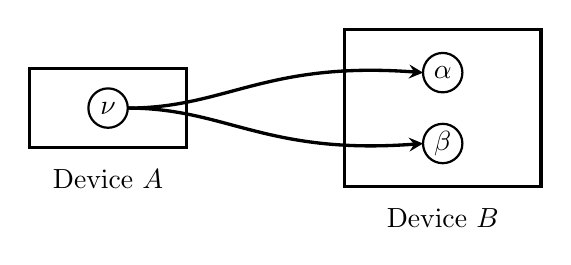
\begin{tikzpicture}
      % Device A
      \draw [very thick] (0, 0) rectangle (2, 1);
      \draw (1, -0.4) node {Device $A$};
      \draw [thick] (1, 0.5) circle [radius=0.25] node {$\nu$};

      % Device B
      \draw [very thick] (4, -0.5) rectangle (6.5, 1.5);
      \draw (5.25, -0.9) node {Device $B$};
      \draw [thick] (5.25, 0.05) circle [radius=0.25] node {$\beta$};
      \draw [thick] (5.25, 0.95) circle [radius=0.25] node {$\alpha$};

      % Edges
      % nu -> beta
      \draw [very thick, -stealth] (1.25, 0.5)
            .. controls (2.5, 0.5) and (3, 1.1)
            ..         (5, 0.95);
      % nu -> alpha
      \draw [very thick, -stealth] (1.25, 0.5)
            .. controls (2.5, 0.5) and (3, -0.1)
            ..          (5, 0.05);
    \end{tikzpicture}
    \caption{}
    \label{fig:cross-a}
  \end{subfigure}
  %
  \begin{subfigure}[b]{0.30\textwidth}
    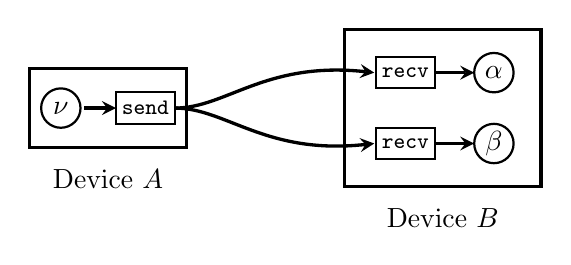
\begin{tikzpicture}
      % Device A
      \draw [very thick] (0, 0) rectangle (2, 1);
      \draw (1, -0.4) node {Device $A$};
      \draw [thick] (0.4, 0.5) circle [radius=0.25] node {$\nu$};

      % Device B
      \draw [very thick] (4, -0.5) rectangle (6.5, 1.5);
      \draw (5.25, -0.9) node {Device $B$};
      \draw [thick] (5.9, 0.05) circle [radius=0.25] node {$\beta$};
      \draw [thick] (5.9, 0.95) circle [radius=0.25] node {$\alpha$};

      % Send Nodes
      \draw [thick] (1.1, 0.3) rectangle ++(0.75, 0.4) node [midway]
      {\footnotesize\texttt{send}};
      \draw [very thick, -stealth] (0.7, 0.5) -- (1.1, 0.5);

      % Receive Nodes
      \draw [thick] (4.4, 0.75) rectangle ++(0.75, 0.4) node [midway]
      {\footnotesize\texttt{recv}};
      \draw [very thick, -stealth] (5.15, 0.95) -- ++(0.5, 0);
      \draw [thick] (4.4, -0.15) rectangle ++(0.75, 0.4) node [midway]
      {\footnotesize\texttt{recv}};
      \draw [very thick, -stealth] (5.15, 0.05) -- ++(0.5, 0);

      % Edges
      % nu -> beta
      \draw [very thick, -stealth] (1.85, 0.5)
            .. controls (2.5, 0.5) and (3, 1.1)
            ..         (4.38, 0.95);
      % nu -> alpha
      \draw [very thick, -stealth] (1.85, 0.5)
            .. controls (2.5, 0.5) and (3, -0.1)
            ..          (4.38, 0.05);
    \end{tikzpicture}
    \caption{}
    \label{fig:cross-b}
  \end{subfigure}
  %
  \begin{subfigure}[h]{0.30\textwidth}
    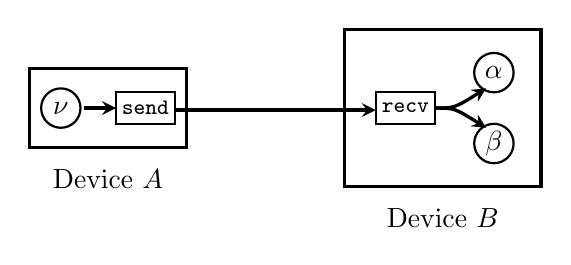
\begin{tikzpicture}
            % Device A
      \draw [very thick] (0, 0) rectangle (2, 1);
      \draw (1, -0.4) node {Device $A$};
      \draw [thick] (0.4, 0.5) circle [radius=0.25] node {$\nu$};

      % Device B
      \draw [very thick] (4, -0.5) rectangle (6.5, 1.5);
      \draw (5.25, -0.9) node {Device $B$};
      \draw [thick] (5.9, 0.05) circle [radius=0.25] node {$\beta$};
      \draw [thick] (5.9, 0.95) circle [radius=0.25] node {$\alpha$};

      % Send Nodes
      \draw [thick] (1.1, 0.3) rectangle ++(0.75, 0.4) node [midway]
      {\footnotesize\texttt{send}};
      \draw [very thick, -stealth] (0.7, 0.5) -- (1.1, 0.5);

      % Receive Nodes
      \draw [thick] (4.4, 0.3) rectangle ++(0.75, 0.4) node [midway]
      {\footnotesize\texttt{recv}};
      \draw [very thick, -stealth] (5.15, 0.5)
                      .. controls +(0.25, 0)
                               .. +(0.65, 0.25);
      \draw [very thick, -stealth] (5.15, 0.5)
                      .. controls +(0.25, 0)
                               .. +(0.65, -0.25);

      % Edges
      \draw [very thick, -stealth] (1.85, 0.475) -- (4.4, 0.475);
    \end{tikzpicture}
    \caption{}
    \label{fig:cross-c}
  \end{subfigure}
  \caption{The three stages of cross-device communication between graph nodes in
    TensorFlow. Figure \ref{fig:cross-a} shows the initial, conceptual
    connections between nodes on different devices. Figure \ref{fig:cross-b}
    gives a more practical overview of how data is actually transmitted across
    devices using \texttt{send} and \texttt{recv} nodes. Lastly, Figure
    \ref{fig:cross-c} shows the final, canonicalized setup, where there is at
    most one \texttt{recv} node per destination device.}
  \label{fig:cross}
\end{figure}

\subsection{Optimizations}\label{sec:model-optim}

To ensure a maximum of efficiency and performance of the TensorFlow execution
model, a number of optimizations are built into the library. In this subsection,
we examine three such improvements: common subgraph elimination, execution
scheduling and finally lossy compression.

\subsubsection{Common Subgraph Elimination}\label{sec:model-optim-common}

An optimization performed by many modern compilers is \emph{common subexpression
  elimination}, whereby a compiler may possibly replace the computation of an
identical value two or more times by a single instance of that computation. The
result is then stored in a temporary variable and reused where it was previously
re-calculated. Similarly, in a TensorFlow graph, it may occur that the same
operation is performed on identical inputs more than once. This can be
inefficient if the computation happens to be an expensive one. Moreover, it may
incur a large memory overhead given that the result of that operation must be
held in memory multiple times. Therefore, TensorFlow also employs a common
subexpression, or, more aptly put, common \emph{subgraph} elimination pass prior
to execution. For this, the computational graph is traversed and every time two
or more operations of the same type (e.g. \texttt{MatMul}) receiving the same
input tensors are encountered, they are canonicalized to only one such
subgraph. The output tensor of that single operation is then redirected to all
dependent nodes. Figure \ref{fig:subgraph-elim} gives an example of common
subgraph elimination.

\begin{figure}
  \centering
  \begin{subfigure}[h]{0.5\textwidth}
    \centering
    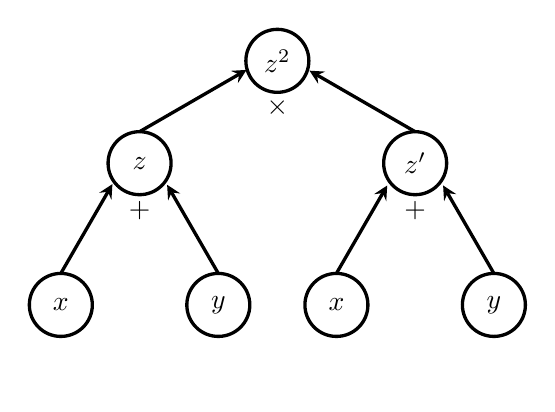
\begin{tikzpicture}
      % First operation
      \draw [very thick] (1, 1.8) circle [radius=0.4cm] node {$z$};

      % Input Nodes
      \draw [very thick] (0, 0) circle [radius=0.4cm] node {$x$};
      \draw [very thick] (2, 0) circle [radius=0.4cm] node {$y$};

      % Edges
      \draw [very thick, -stealth] (0, 0.4) -- ++(60:1.31);
      \draw [very thick, -stealth] (2, 0.4) -- ++(120:1.3);

      % Operation Label
      \draw (1, 1.2) node {$+$};

      % Second operation
      \draw [very thick] (4.5, 1.8) circle [radius=0.4cm] node {$z'$};

      % Input Nodes
      \draw [very thick] (3.5, 0) circle [radius=0.4cm] node {$x$};
      \draw [very thick] (5.5, 0) circle [radius=0.4cm] node {$y$};

      % Edges
      \draw [very thick, -stealth] (3.5, 0.4) -- ++(60:1.29);
      \draw [very thick, -stealth] (5.5, 0.4) -- ++(120:1.29);

      % Operation Label
      \draw (4.5, 1.2) node {$+$};

      % Square
      \draw [very thick] (2.75, 3.1) circle [radius=0.4cm] node {$z^2$};

      % Edges
      \draw [very thick, -stealth] (1, 2.2) -- ++(30:1.57);
      \draw [very thick, -stealth] (4.5, 2.2) -- ++(150:1.55);

      % Operation Label
      \draw (2.75, 2.5) node {$\times$};

      % Spacing fuck you
      \draw (0, -1);
    \end{tikzpicture}
  \end{subfigure}
  %
  \begin{subfigure}[h]{0.5\textwidth}
    \centering
    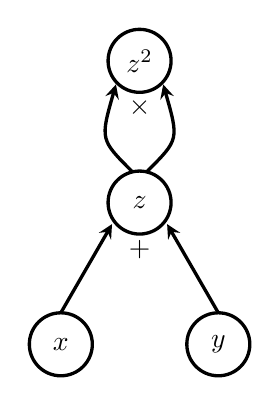
\begin{tikzpicture}
      % First operation
      \draw [very thick] (1, 1.8) circle [radius=0.4cm] node {$z$};

      % Input Nodes
      \draw [very thick] (0, 0) circle [radius=0.4cm] node {$x$};
      \draw [very thick] (2, 0) circle [radius=0.4cm] node {$y$};

      % Edges
      \draw [very thick, -stealth] (0, 0.4) -- ++(60:1.3);
      \draw [very thick, -stealth] (2, 0.4) -- ++(120:1.3);

      % Operation Label
      \draw (1, 1.2) node {$+$};

      % Square
      \draw [very thick] (1, 3.6) circle [radius=0.4cm] node {$z^2$};

      % Operation Label
      \draw (1, 3) node {$\times$};

      % Edges
      \draw [very thick, -stealth] (0.9, 2.2) .. controls +(-0.4, 0.4) .. +(-0.2, 1.1);
      \draw [very thick, -stealth] (1.1, 2.2) .. controls +(+0.4, 0.4) .. +(+0.2, 1.1);
    \end{tikzpicture}
  \end{subfigure}
  \caption{An example of how common subgraph elimination is used to transform the
    equations $z = x + y$, $z' = x + y$, $z^2 = z \cdot z'$ to just two
    equations $z = x + y$ and $z^2 = z \cdot z$. This computation could
    theoretically be optimized further to a \texttt{square} operation requiring
    only one input (thus reducing the cost of data movement), though it is not
    known if TensorFlow employs such secondary canonicalization.}
  \label{fig:subgraph-elim}
\end{figure}

\subsubsection{Scheduling}\label{sec:model-optim-schedule}

A simple yet powerful optimization is to schedule node execution as late as
possible. Ensuring that the results of operations remain in memory only for the
minimum required amount of time reduces peak memory consumption and can thus
greatly improve the overall performance of the system. The authors of
\cite{tensorflow} note that this is especially vital on devices such as GPUs,
where memory resources are scarce. Furthermore, careful scheduling also pertains
to the activation of \texttt{send} and \texttt{recv} nodes, where not only
memory but also network resources are contested.

\subsubsection{Lossy Compression}\label{sec:model-optim-lossy}

One of the primary goals of many machine learning algorithms used for
classification, recognition or other tasks is to build robust models. With
\emph{robust} we mean that an optimally trained model should ideally not change
its response if it is first fed a signal and then a noisy variation of that
signal. As such, these machine learning algorithms typically do not require high
precision arithmetic as provided by standard IEEE 754 32-bit floating point
values. Rather, 16 bits of precision in the mantissa would do just as well. For
this reason, another optimization performed by TensorFlow is the internal
addition of conversion nodes to the computational graph, which convert such
high-precision 32-bit floating-point values to truncated 16-bit representations
when communicating across devices and across machines. On the receiving end, the
truncated representation is converted back to 32 bits simply by filling in
zeros, rather than rounding \cite{tensorflow}.

\subsection{Additions to the Basic Programming Model}\label{sec:model-ext}

Having discussed the basic computational paradigms and execution model of
TensorFlow, we will now review three more advanced topics that we deem highly
relevant for anyone wishing to use TensorFlow to create machine learning
algorithms. First, we discuss how TensorFlow handles \emph{gradient
  back-propagation}, an essential concept for many deep learning
applications. Then, we study how TensorFlow graphs support \emph{control
  flow}. Lastly, we briefly touch upon the topic of \emph{checkpoints}, as they
are very useful for maintenance of large models.

\subsubsection{Back-Propagation Nodes}\label{sec:model-ext-backprop}

In a large number of deep learning and other machine learning algorithms, it is
necessary to compute the gradients of particular nodes of the computational
graph with respect to one or many other nodes. For example, in a neural network,
we may compute the cost $c$ of the model for a given example $x$ by passing that
example through a series of non-linear transformations. If the neural network
consists of two hidden layers represented by functions $f(x;w) = f_x(w)$ and
$g(x;w) = g_x(w)$ with internal weights $w$, we can express the cost for that
example as $c = (f_x \circ g_x)(w) = f_x(g_x(w))$. We would then typically
calculate the gradient $dc/dw$ of that cost with respect to the weights and use
it to update $w$. Often, this is done by means of the \emph{back-propagation}
algorithm, which traverses the graph in reverse to compute the chain rule
$[f_x(g_x(w))]' = f_x'(g_x(w)) \cdot g_x'(w)$.

In \cite{goodfellow2016}, two approaches for back-propagating gradients through
a computational graph are described. The first, which the authors refer to as
\emph{symbol-to-number differentiation}, receives a set of input values and then
computes the \emph{numerical values} of the gradients at those input values. It
does so by explicitly traversing the graph first in the forward order
(forward-propagation) to compute the cost, then in reverse order
(back-propagation) to compute the gradients via the chain rule. Another
approach, more relevant to TensorFlow, is what \cite{goodfellow2016} calls
\emph{symbol-to-symbol derivatives} and \cite{tensorflow} terms \emph{automatic
  gradient computation}. In this case, gradients are not computed by an explicit
implementation of the back-propagation algorithm. Rather, special nodes are added
to the computational graph that calculate the gradient of each operation and
thus ultimately the chain rule. To perform back-propagation, these nodes must
then simply be executed like any other nodes by the graph evaluation engine. As
such, this approach does not produce the desired derivatives as a numeric value,
but only as a \emph{symbolic handle} to compute those values.

When TensorFlow needs to compute the gradient of a particular node $\nu$ with
respect to some other tensor $\alpha$, it traverses the graph in reverse order
from $\nu$ to $\alpha$. Each operation $o$ encountered during this traversal
represents a function depending on $\alpha$ and is one of the ``links'' in the
chain $(\nu \,\circ\, \dots\, \circ\, o \,\circ\, \dots)(\alpha)$ producing the
output tensor of the graph. Therefore, TensorFlow adds a \emph{gradient node}
for each such operation $o$ that takes the gradient of the previous link (the
outer function) and multiplies it with its own gradient. At the end of the
traversal, there will be a node providing a symbolic handle to the overall
target derivative $\frac{d\nu}{d\alpha}$, which \emph{implicitly} implements the
back-propagation algorithm. It should now be clear that back-propagation in this
symbol-to-symbol approach is \emph{just another operation}, requiring no
exceptional handling. Figure \ref{fig:gradients} shows how a computational graph
may look before and after gradient nodes are added.

\begin{figure}
  \centering
  \begin{subfigure}[b]{0.2\textwidth}
    \centering
    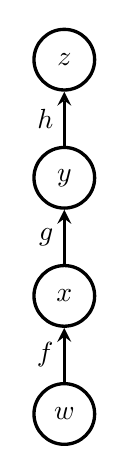
\begin{tikzpicture}
      % Nodes
      \path [very thick] (0, 0)
            coordinate [draw, circle, text width=0.5cm] (w) node {$w$};
      \path [very thick] (0, 1.5)
             coordinate [draw, circle, text width=0.5cm] (x) node {$x$};
      \path [very thick] (0, 3)
            coordinate [draw, circle, text width=0.5cm] (y) node {$y$};
      \path [very thick] (0, 4.5)
            coordinate [draw, circle, text width=0.5cm] (z) node {$z$};

      % Edges
      \draw [very thick, -stealth] (w) -- (x) node [midway, left] {$f$};
      \draw [very thick, -stealth] (x) -- (y) node [midway, left] {$g$};
      \draw [very thick, -stealth] (y) -- (z) node [midway, left] {$h$};
    \end{tikzpicture}
    \caption{}
    \label{fig:gradients-a}
  \end{subfigure}
  \begin{subfigure}[b]{0.2\textwidth}
    \centering
    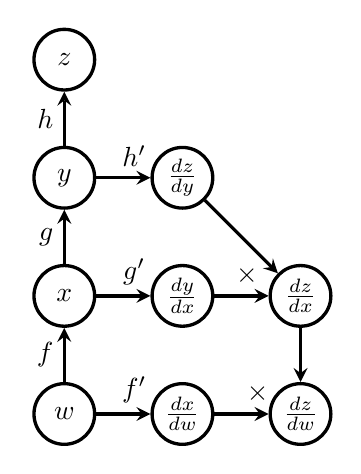
\begin{tikzpicture}
      % Nodes
      \path [very thick] (0, 0)
            coordinate [draw, circle, text width=0.5cm] (w) node {$w$};
      \path [very thick] (0, 1.5)
             coordinate [draw, circle, text width=0.5cm] (x) node {$x$};
      \path [very thick] (0, 3)
            coordinate [draw, circle, text width=0.5cm] (y) node {$y$};
      \path [very thick] (0, 4.5)
            coordinate [draw, circle, text width=0.5cm] (z) node {$z$};

      % Edges
      \draw [very thick, -stealth] (w) -- (x) node [midway, left] {$f$};
      \draw [very thick, -stealth] (x) -- (y) node [midway, left] {$g$};
      \draw [very thick, -stealth] (y) -- (z) node [midway, left] {$h$};

      % Derivatives
      \path [very thick] (1.5, 0)
            coordinate [draw, circle, text width=0.5cm] (wp) node {$\frac{dx}{dw}$};
      \path [very thick] (1.5, 1.5)
             coordinate [draw, circle, text width=0.5cm] (xp) node {$\frac{dy}{dx}$};
      \path [very thick] (1.5, 3)
            coordinate [draw, circle, text width=0.5cm] (yp) node {$\frac{dz}{dy}$};

      % Edges
      \draw [very thick, -stealth] (w) -- (wp) node [pos=0.7, above] {$f'$};
      \draw [very thick, -stealth] (x) -- (xp) node [pos=0.7, above] {$g'$};
      \draw [very thick, -stealth] (y) -- (yp) node [pos=0.7, above] {$h'$};

     % Chain Rule
      \path [very thick] (3, 0)
            coordinate [draw, circle, text width=0.5cm]
            (dzdw) node {$\frac{dz}{dw}$};
      \path [very thick] (3, 1.5)
             coordinate [draw, circle, text width=0.5cm]
             (dzdx) node {$\frac{dz}{dx}$};

      % Edges
      \draw [very thick, -stealth] (wp) -- (dzdw)
            node [pos=0.8, above] {$\times$};
      \draw [very thick, -stealth] (xp) -- (dzdx)
            node [pos=0.6, above] {$\times$};
      \draw [very thick, -stealth] (yp) -- (dzdx);
      \draw [very thick, -stealth] (dzdx) -- (dzdw);
    \end{tikzpicture}
    \caption{}
    \label{fig:gradients-b}
  \end{subfigure}
  \caption{A computational graph before (\ref{fig:gradients-a}) and after
    (\ref{fig:gradients-b}) gradient nodes are added. In this
    \emph{symbol-to-symbol} approach, the gradient $\frac{dz}{dw}$ is just
    simply an operation like any other and therefore requires no special
    handling by the graph evaluation engine.}
  \label{fig:gradients}
\end{figure}

In \cite{tensorflow} it is noted that symbol-to-symbol derivatives may incur a
considerable performance cost and especially result in increased memory
overhead. To see why, it is important to understand that there exist two
equivalent formulations of the chain rule. The first reuses previous
computations and therefore requires them to be stored longer than strictly
necessary for forward-propagation. For arbitrary functions $f$, $g$ and $h$ it is
given in Equation \ref{eq:chain-reuse}:
\begin{equation}\label{eq:chain-reuse}
  \frac{\mathrm{d} f}{\mathrm{d} w} = f'(y) \cdot g'(x) \cdot h'(w) \text{ with } y = g(x), x =
  h(w)
\end{equation}
The second possibility for computing the chain rule was already shown, where
each function recomputes all of its arguments and invokes every function it
depends on. It is given in Equation \ref{eq:chain-recomp} for reference:
\begin{equation}\label{eq:chain-recomp}
  \frac{\mathrm{d} f}{\mathrm{d} w} = f'(g(h(w))) \cdot g'(h(w)) \cdot h'(w)
\end{equation}
According to \cite{tensorflow}, TensorFlow currently employs the first
approach. Given that the inner-most functions must be recomputed for almost
every link of the chain if this approach is not employed, and taking into
consideration that this chain may consist of many hundreds or thousands of
operations, this choice seems sensible. However, on the flip side, keeping
tensors in memory for long periods of time is also not optimal, especially on
devices like GPUs where memory resources are scarce. For Equation
\ref{eq:chain-recomp}, memory held by tensors could in theory be freed as soon
as it has been processed by its graph dependencies. For this reason, in
\cite{tensorflow} the development team of TensorFlow states that recomputing
certain tensors rather than keeping them in memory may be a possible performance
improvement for the future.

\subsubsection{Control Flow}\label{sec:model-ext-flow}

Some machine learning algorithms may benefit from being able to control the flow
of their execution, performing certain steps only under a particular condition
or repeating some computation a fixed or variable number of times. For this,
TensorFlow provides a set of control flow primitives including
\texttt{if}-conditionals and \texttt{while}-loops. The possibility of loops is
the reason why a TensorFlow computational graph is not necessarily
\emph{acyclic}. If the number of iterations for of a loop would be fixed and
known at graph compile-time, its body could be \emph{unrolled} into an acyclic
sequence of computations, one per loop iteration \cite{theano}. However, to
support a variable amount of iterations, TensorFlow is forced to jump through an
additional set of hoops, as described in \cite{tensorflow}.

One aspect that must be especially cared for when introducing control flow is
back-propagation. In the case of a conditional, where an \texttt{if}-operation
returns either one or the other tensor, it must be known which branch was taken
by the node during forward-propagation so that gradient nodes are added only to
this branch. Moreover, when a loop body (which may be a small graph) was
executed a certain number of times, the gradient computation does not only need
to know the number of iterations performed, but also requires access to each
intermediary value produced. This technique of stepping through a loop in
reverse to compute the gradients is referred to as \emph{back-propagation
  through time} in \cite{theano}.

\subsubsection{Checkpoints}\label{sec:model-ext-check}

Another extension to TensorFlow's basic programming model is the notion of
\emph{checkpoints}, which allow for persistent storage and recovery of
variables. It is possible to add \texttt{Save} nodes to the computational graph
and connect them to variables whose tensors you wish to serialize. Furthermore,
a variable may be connected to a \texttt{Restore} operation, which deserializes
a stored tensor at a later point. This is especially useful when training a
model over a long period of time to keep track of the model's performance while
reducing the risk of losing any progress made. Also, checkpoints are a vital
element to ensuring fault tolerance in a distributed environment
\cite{tensorflow}.

%%% Local Variables:
%%% mode: latex
%%% TeX-master: "../paper"
%%% End: